\documentclass{article}
\usepackage{geometry}
\geometry{margin=0.8in}
\usepackage[subpreambles=true]{standalone}
\usepackage[T1]{fontenc}
\usepackage[utf8]{inputenc}
\usepackage[english, danish]{babel}
\usepackage{graphicx,wrapfig,lipsum}
\usepackage{float}
\usepackage{hyperref}
\usepackage{enumitem}
\usepackage{tgbonum}
\usepackage{import}
\newcommand{\myparagraph}[1]{\paragraph{#1}\mbox{}\\}
\newcommand{\mysubparagraph}[1]{\subparagraph{#1}\mbox{}\\}
\usepackage{xcolor}
\usepackage{ulem}
\usepackage{comment}
\usepackage{pdfpages}
\usepackage[backend=bibtex, style=numeric]{biblatex}
\addbibresource{references.bib}

\newcommand\myworries[1]{\textcolor{red}{#1}}

%\title{Final CDIO}
%\author{}
%\date{Januar 2018}
\begin{document}
{\fontfamily{phv}\selectfont
%\maketitle
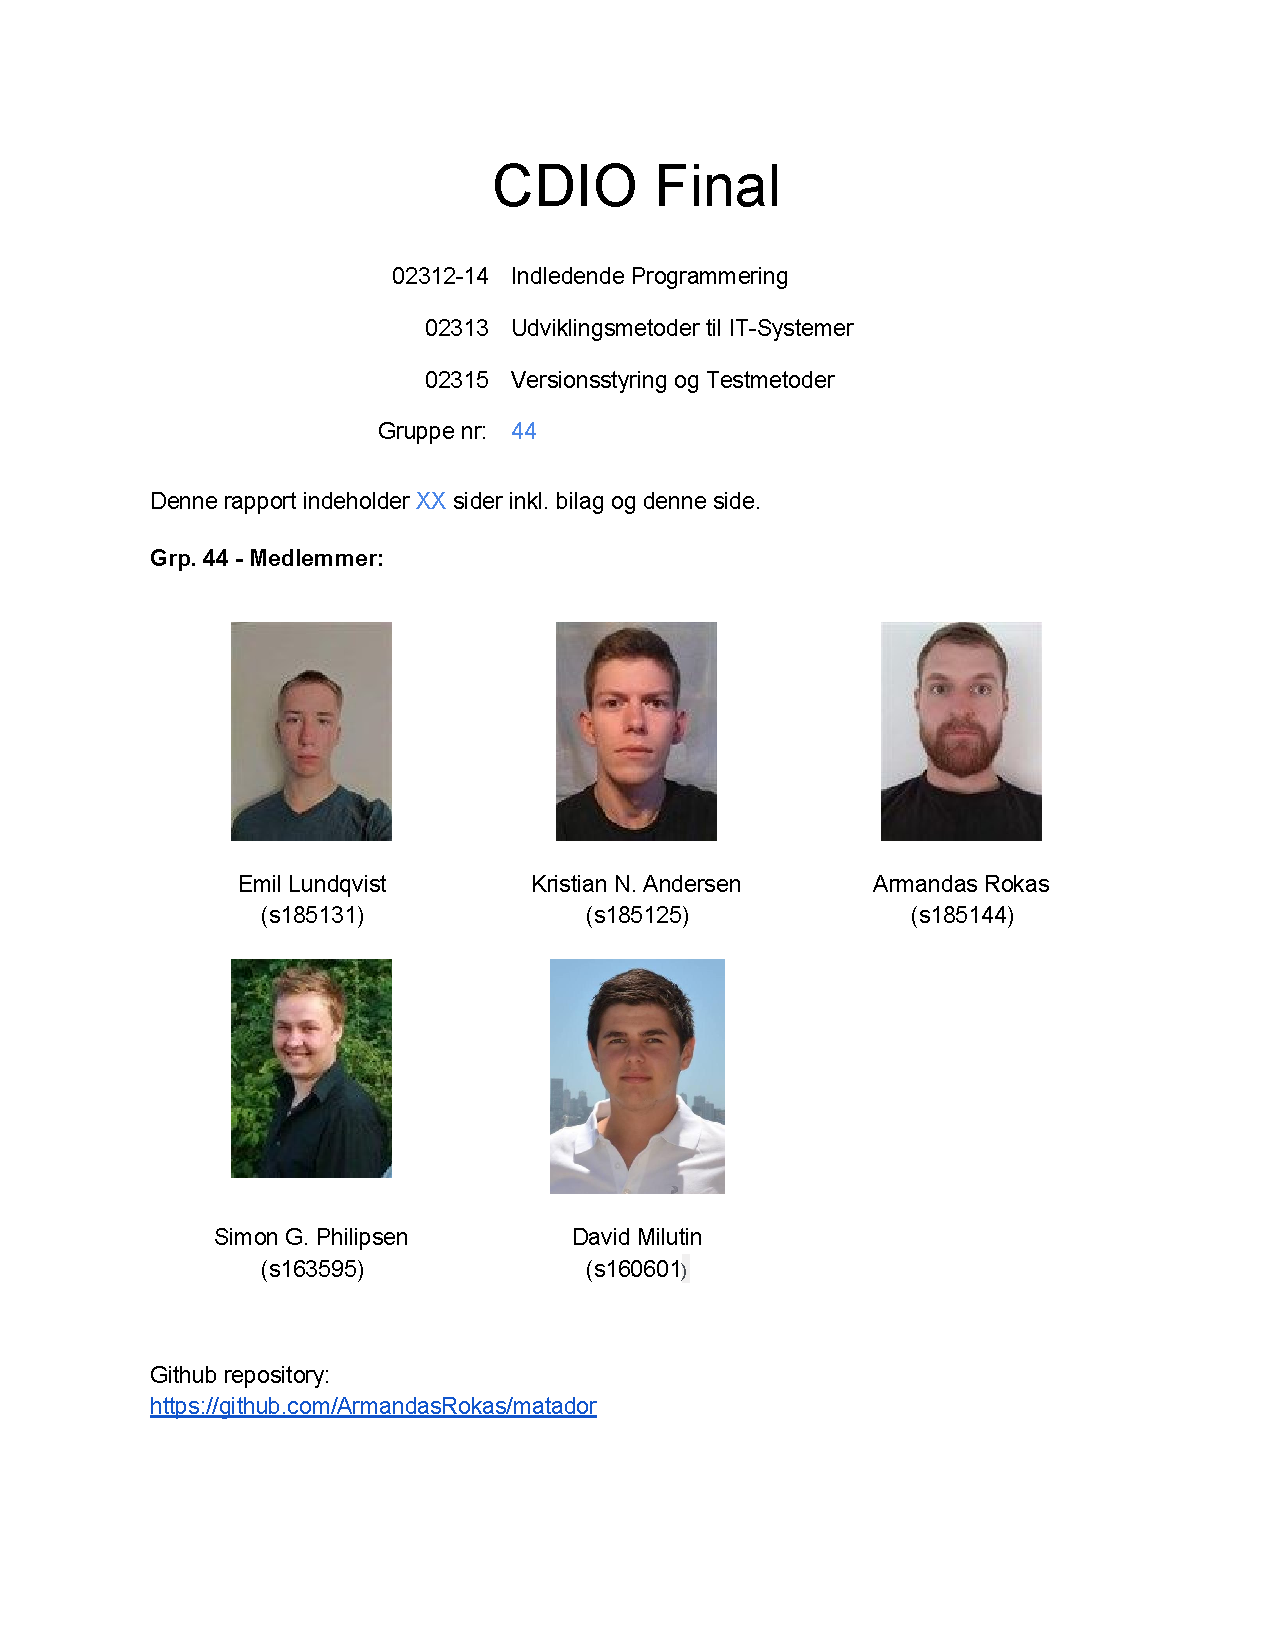
\includepdf[page={1}]{sections/front_page}
\thispagestyle{empty}
\newpage
\section*{Abstract}
\import{sections/}{abstract}
\thispagestyle{empty}
\newpage
\tableofcontents
\thispagestyle{empty}
\newpage
\clearpage
\setcounter{page}{1}

\section{Introduktion}
\import{sections/}{introduction}

\section{Analyse}
\subsection{Vision}
\import{sections/}{vision}

\subsection{Interessent- og aktøranalyse}
\import{artifacts/}{interessent_analyse}
\subsection{Kravspecifikation}
\import{artifacts/}{kravliste}

\subsection{Use case diagram}
\import{artifacts/}{use_case_diagram}
\newpage
\subsection{Use case beskrivelser}
\import{use_cases/}{UC1_opret_spillere}
\import{use_cases/}{UC11_kast_terninger}
%\import{use_cases/}{UC1_spil_spillet}
\import{use_cases/}{UC2_koeb_grund}
\import{use_cases/}{UC3_kom_ud_af_faengsel}
\import{use_cases/}{UC4_proev_lykken}
\import{use_cases/}{UC5_pantsaette_hus}
\import{use_cases/}{UC6_ophaeve_pantsaetning}
\import{use_cases/}{UC7_saelge_ejendom}
\import{use_cases/}{UC8_byg_hus}
\import{use_cases/}{UC9_byg_hotel}
\import{use_cases/}{UC10_gaa_fallit}
\newpage
\subsection{Domænmodel}
\import{artifacts/}{domain_model}
\newpage
%\subsection{Systemssekvensdiagram}

%\newpage
\section{Design}

\subsection{Pakkediagram}
\import{artifacts/}{pakkediagram}
\newpage
\subsection{Sekvensdiagrammer}
%\newpage
\subsection{Klassediagram}
%\import{artifacts/}{DKD}

\section{Implementering}
\subsection{Kodeprocessen}
\import{sections/}{kodeprocessen}
\subsection{Visitor pattern}
\import{sections/}{visitor_pattern}
\section{Testing}
\subsection{Unit testing}
\import{test_cases/}{TC1_setNumberOfSiblingTest}
\subsection{Itegration testing}

\subsection{Acceptance testing}
\import{test_cases/}{acceptence_test}

\section{Konklution}
\import{sections/}{konklusion}
test

\newpage
\section*{Ordbog}
\addcontentsline{toc}{section}{Ordbog}

\import{artifacts/}{ordbog}




\newpage
\cleardoublepage
\printbibliography[heading=bibintoc]
}

\end{document}